% +------------------------------------------------------------------------+
% | Reference manual page: Triangulation_data_structure_2.tex
% +------------------------------------------------------------------------+
% | 07.04.2000   Author
% | Package: Package
% | 
\RCSdef{\RCSTriangulationdatastructureRev}{$Id$}
\RCSdefDate{\RCSTriangulationdatastructureDate}{$Date$}
% |
%%RefPage: end of header, begin of main body
% +------------------------------------------------------------------------+

\begin{ccRefConcept}{TriangulationDataStructure_2}

%% \ccHtmlCrossLink{}     %% add further rules for cross referencing links
%% \ccHtmlIndexC[concept]{} %% add further index entries
\ccCreationVariable{tds}
\ccDefinition
  
The concept \ccRefName\ describes the requirements  for
the second template parameter of the basic triangulation class
\ccc{Triangulation_2<Traits,Tds>} and of all other 2D triangulation classes.

The concept can be seen as a container for the 
faces and vertices of the triangulation.
The concept \ccRefName\  includes two sub-concepts
\ccc{TriangulationDataStructure_2::Vertex} and
\ccc{TriangulationDataStructure_2::Face}\lcTex{, 
described respectively \ccRefPage{TriangulationDataStructure_2::Vertex}
and \ccRefPage{TriangulationDataStructure_2::Face}}. 

The \ccRefName\ 
maintains incidence and adjacency relations
among vertices and faces.

Each triangular face gives access to its three incident vertices 
and to its three adjacent faces. 
Each vertex gives access to one of its incident faces
and through that face to the circular list of its incident faces.

The three vertices of a face are indexed with 0, 1 and 2.
The neighbors of a face are also 
indexed with 0,1,2 in such a way that the neighbor indexed by \ccc{i}
is opposite to the vertex with the same index.

Each edge has two implicit representations : the edge
of a face \ccc{f}  which is opposed to the vertex indexed \ccc{i},
can be represented as well as an edge of the \ccc{neighbor(i)} of 
\ccc{f}. See Figure~\ref{2D_Triangulation_Fig_neighbors1}


The triangulation data structure
 is responsible for  the combinatorial integrity of the triangulation.
This means that the triangulation data structure
allows to perform some combinatorial operations
on the triangulation and guarantees the maintenance on 
proper incidence and adjacency relations among the vertices
and faces. The term combinatorial operations
 means that those operations are purely topological
and do not depend on the geometric embedding.
Insertion of a new vertex in a given face, or in a given edge,
suppression of a vertex of degree three,  flip of two edges
are examples of combinatorial operations.



\ccTypes
\ccThree{typedef std::pair<Face_handle,int>xxxxx}{Edge; }{}
\ccThreeToTwo

\ccNestedType{size_type}{Size type (unsigned integral type)}
\ccGlue
\ccNestedType{difference_type}{Difference type (signed integral type)}

\ccNestedType{Vertex} { The vertex type. Requirements for this type
are described in concept \ccc{TriangulationDataStructure_2::Vertex}
\lcTex{\ccRefPage{TriangulationDataStructure_2::Vertex}}.}
\ccGlue
\ccNestedType{Face}{The face type. Requirements for this type
are described in concept \ccc{TriangulationDataStructure_2::Face}
\lcTex{\ccRefPage{TriangulationDataStructure_2::Face}}.}

Vertices and faces are accessed  via \ccc{Vertex_handle} and
\ccc{Face_handle}. These types 
are models of the concept \ccc{Handles} which basically
supports the two dereference operators \ccc{*} and \ccc{->}.

\ccNestedType{Vertex_handle}{Handle to a vertex}
\ccGlue
\ccNestedType{Face_handle}{Handle to a face.}

\begin{ccAdvanced}
\ccNestedType{template <typename Vb2> struct Rebind_vertex}
{This nested template class allows to get the type of a triangulation
data structure that only changes the vertex type.  It has to define a type
\ccc{Other} which is a {\it rebound} triangulation data structure, that is, the
one whose \ccc{TriangulationDSVertexBase_2} will be \ccc{Vb2}.}
\ccGlue
\ccNestedType{template <typename Fb2> struct Rebind_face}
{This nested template class allows to get the type of a triangulation
data structure that only changes the face type.  It has to define a type
\ccc{Other} which is a {\it rebound} triangulation data structure, that is, the
one whose \ccc{TriangulationDSFaceBase_2} will be \ccc{Fb2}.}
\end{ccAdvanced}


\ccTypedef{typedef std::pair<Face_handle,int> Edge;}{The edge type.
The \ccc{Edge(f,i)} is edge common to faces \ccc{f} and 
\ccc{f.neighbor(i)}. It is also the edge joining the vertices
\ccc{vertex(cw(i))} and \ccc{vertex(ccw(i))} of \ccc{f}.}


The following iterators allow one to visit all the vertices, edges
and  faces
of a triangulation data structure. They are all
bidirectional, non-mutable iterators.

\ccNestedType{Face_iterator}{}
\ccGlue
\ccNestedType{Edge_iterator}{}
\ccGlue
\ccNestedType{Vertex_iterator}{}


The following circulators allow to visit all the edges or faces
incident to a given vertex and all the vertices
adjacent to a given vertex.  They are all bidirectional and non
mutable.

\ccNestedType{Face_circulator}{}
\ccGlue
\ccNestedType{Edge_circulator}{}
\ccGlue
\ccNestedType{Vertex_circulator}{}
 
Iterators and circulators are convertible to the corresponding handles, thus
they can be passed directly as argument
to the functions expecting a handle.




\ccCreation
\ccCreationVariable{tds}  %% choose variable name
\ccThree{TriangulationDataStructure_2& }{tds.swap}{}
\ccThreeToTwo

\ccConstructor{TriangulationDataStructure_2();}{default constructor.}

\ccConstructor{TriangulationDataStructure_2( const
TriangulationDataStructure_2& tds1)}
{Copy constructor. All the vertices and faces are duplicated.}

\ccMethod{TriangulationDataStructure_2& operator=( const
TriangulationDataStructure_2& tds1);}
{Assignment. All the vertices and faces of \ccc{tds1} are duplicated
in \ccVar\ . Former faces and vertices of \ccVar\ , if any, are
deleted}

\ccThree{Vertex_handle }{tds.insert_in_facet}{}

\ccMethod{Vertex_handle
copy_tds(const TriangulationDataStructure_2 & tds1, 
         Vertex_handle v = Vertex_handle());}
{\ccc{tds1} is copied into \ccVar. If $v\, !\!= NULL$, the vertex of \ccVar\ 
corresponding to \ccc{v} is returned, otherwise \ccc{Vertex_handle()} 
is returned.
\ccPrecond{The optional argument \ccc{v} is a vertex of \ccc{tds1}.}}

\ccMethod{void swap( TriangulationDataStructure_2 &  tds1);}
{Swaps \ccVar\ and \ccc{tds1}. Should be preferred to \ccVar=\ccc{tds1} or \ccVar(\ccc{tds1})
when \ccc{tds1} is deleted after that.}
\ccMethod{void clear();}{Deletes all faces and all finite vertices.}
%\ccGlue
%\ccModifierCrossRefOff
%\ccFunction{void ~TriangulationDataStructure_2();}
%{Destructor. All vertices and faces are deleted.}
%\ccModifierCrossRefOff

\ccAccessFunctions
\ccThree{void}{tds.set_number_of_vertices(size_type n)}{}
\ccMethod{int dimension() const;}
{returns the dimension of the triangulation.}
\ccGlue
\ccMethod{size_type number_of_vertices() const;}
{returns the number of vertices in the data structure.}
\ccGlue
\ccMethod{size_type number_of_faces() const ;}
{returns the number of two dimensional faces in the data structure.}
\ccGlue
\ccMethod{size_type number_of_edges() const;}
{returns the number of edges  in the triangulation data structure.}
\ccGlue
\ccMethod{size_type number_of_full_dim_faces() const;}
{returns the  number of full dimensional faces, 
i.e. faces of dimension equal to the dimension
of the triangulation. This is the actual
number of faces stored in the triangulation data structure.}

\begin{ccAdvanced}
\ccHeading{Setting}
\ccMethod{void set_dimension (int n);}{sets the dimension.}
\end{ccAdvanced}

\ccHeading{Queries}
\ccThree{bool}{is_edge(Face_handle fh, int i)}{}

\ccMethod{bool is_vertex(Vertex_handle v) const;}{returns true if
\ccc{v} is a vertex of \ccVar.}
\ccGlue
\ccMethod{bool is_edge(Face_handle fh, int i) const;}
{tests whether \ccc{(fh,i)} is an edge of \ccVar. Answers \ccc{false} when
\ccc{dimension()} $<1$ .}
\ccGlue
\ccMethod{bool is_edge(Vertex_handle va, Vertex_handle vb) const;}{returns true if
\ccc{va vb} is an edge of \ccVar.}
\ccGlue
\ccMethod{bool is_edge(Vertex_handle va, Vertex_handle vb, Face_handle &fr,
int &i) const;}{as previous. In addition, if true is returned
\ccc{fr} and \ccc{i} are set such that the pair \ccc{(fr,i)}
is the description 
of  the ordered edge \ccc{va vb}.}
\ccGlue
\ccMethod{bool is_face(Face_handle fh) const;}
{tests whether \ccc{fh} is a face of \ccVar. Answers \ccc{false} when
\ccc{dimension()} $<2$ .}
\ccGlue
\ccMethod{bool is_face(Vertex_handle v1, Vertex_handle v2,
Vertex_handle v3) 
const;}{\ccc{true} if there is a face having \ccc{v1}, \ccc{v2} and\ccc{v3} 
as vertices.}
\ccGlue
\ccMethod{bool is_face(Vertex_handle v1, Vertex_handle v2, Vertex_handle v3,
      Face_handle &fr) const;}{as above. In addition, if \ccc{true} is returned, fr is a pointer
to the face with  \ccc{v1}, \ccc{v2} and \ccc{v3} 
as vertices.}

\ccHeading{Traversing the triangulation}
\ccThree{Vertex_iterator}{tds.number_of_faces()x}{}
\ccMethod{Face_iterator faces_begin() const;}{visits all faces}
\ccGlue
\ccMethod{Face_iterator faces_end() const;}{}
\ccGlue
\ccMethod{Vertex_iterator vertices_begin() const;}{visits all vertices}
\ccGlue
\ccMethod{Vertex_iterator vertices_end() const;}{}
\ccGlue
\ccMethod{Edge_iterator edges_begin() const;}{visits all edges}
\ccGlue
\ccMethod{ Edge_iterator edges_end() const;}{}

\ccThree{Vertex_circulator}{tds.number_of_faces()x}{}
Three circulator classes allow to traverse the edges or faces
incident to a vertex or the vertices adjacent to this vertex..
A face circulator is invalidated by any modification of the face it
points to. An edge circulator is invalidated
by any modification of anyone of the two faces incident to the edge
pointed to.  A vertex circulator that turns around vertex \ccc{v}
and that has as value a pointer to vertex \ccc{w}, is invalidated
by any modification of anyone of the two faces incident to \ccc{v}
and \ccc{w}.

\ccMethod{Vertex_circulator
          incident_vertices(Vertex_handle v, Face_handle f=NULL)
const;}
{\ccPrecond If the
face \ccc{f} is given, it has to be incident to be a face of \ccVar\ 
incident to \ccc{v} 
and the circulator begins with 
the vertex \ccc{f->vertex(ccw(i))} 
if \ccc{i} is the index of \ccc{v}  in \ccc{f}.} 
\ccGlue
\ccMethod{Edge_circulator
          incident_edges(Vertex_handle v, Face_handle f=NULL) const;}
{\ccPrecond If the
face \ccc{f} is given, it has to be a face of \ccVar\ 
incident to \ccc{v} 
and the circulator begins with 
the edge \ccc{(f,cw(i))} of \ccc{f}
if  \ccc{i} is the index of \ccc{v}  in \ccc{f}.}
\ccGlue
\ccMethod{Face_circulator
          incident_faces(Vertex_handle v, Face_handle f=NULL) const;}
{\ccPrecond If the
face \ccc{f} is given, it has to be a face of \ccVar\ 
incident to \ccc{v} 
and the circulator begins with the face
\ccc{f}.}

\ccMethod{Vertex_handle  mirror_vertex(Face_handle f, int i) const;}{returns vertex of \ccc{f->neighbor(i)}.}

\ccMethod{int   mirror_index(Face_handle f, int i) const;}{returns the index of \ccc{f} as a neighbor of \ccc{f->neighbor(i)}.}

\ccMethod{Edge   mirror_edge(Edge e) const;}{returns the same edge seen from the other adjacent face.}

\ccHeading{Modifiers}
The following modifier member functions  guarantee
the combinatorial validity of the resulting triangulation.

\ccThree{void}{tds.flip(Face_handle f, int i);}{}
\ccMethod{void flip(Face_handle f, int i);}{exchanges the edge incident to
\ccc{f} and \ccc{f->neighbor(i)} with the other
diagonal of the quadrilateral formed by \ccc{f} and  \ccc{f->neighbor(i)}.}


\begin{figure}
\begin{ccTexOnly}
\begin{center} %\IpeScale{70} \Ipe{Triangulation_2/Flip.ipe} \end{center}
\input{Triangulation_2/flip.ltex}
\end{center}
\end{ccTexOnly} 
\caption{Flip.
\label{I1_fig_flip}}

\begin{ccHtmlOnly}
<CENTER>
<img border=0 src="Flip.gif" align=middle alt="Flip">
</CENTER>
\end{ccHtmlOnly} 
\end{figure}

\ccThree{Vertex_handle}{tds.insert_in_edge(Face_handle f, int i);}{}
\ccMethod{Vertex_handle  insert_first();} {creates the first 
vertex and returns a pointer to it.}
\ccGlue
\ccMethod{Vertex_handle  insert_second();} {creates the second 
vertex and returns a pointer to it.}
\ccMethod{Vertex_handle  insert_in_edge(Face_handle f, int i);} {adds a
vertex \ccc{v} splitting 
edge \ccc{i} of face \ccc{f}. Return a  pointer to \ccc{v}.}
\ccGlue
\ccMethod{Vertex_handle  insert_in_face(Face_handle f);} {adds a vertex
\ccc{v} splitting  face
\ccc{f} in three. Face \ccc{f} is modified,
two new faces are created. Return a  pointer to \ccc{v} }
\ccGlue
\ccMethod{Vertex_handle  insert_dim_up(Vertex_handle  w, bool
orient=true);} 
{adds
a vertex \ccc{v}, increasing by one the dimension of the triangulation.
Vertex \ccc{v} and the existing vertex \ccc{w} are linked to all 
the vertices of the triangulation. 
The Boolean \ccc{orient} decides the final orientation of all 
faces. A pointer to vertex \ccc{v} is returned.
}

\begin{figure}
\begin{ccTexOnly}
%\begin{center} \IpeScale{70} \Ipe{Triangulation_2/Three.ipe} \end{center}
\begin{center} \input{Triangulation_2/insert.ltex} \end{center}
\caption{Insertion}
\end{ccTexOnly} 

\begin{ccHtmlOnly}
<CENTER>
<img border=0 src="Three.gif" align=middle alt="Insertion">
</CENTER>
\end{ccHtmlOnly} 
\end{figure}


\ccThree{void}{tds.remove_dim_down(Vertex_handle  v);}{}
\ccMethod{void remove_degree_3(Vertex_handle  v, Face *f=NULL);}
{removes a vertex of degree 3. Two of the incident faces are destroyed,
the third one is modified.
If parameter \ccc{f}  is specified, it has to be a face incident to \ccc{v}
and will be the modified face.
\ccPrecond{Vertex
\ccc{v} is a finite vertex with degree 3
and, if specified, face \ccc{f} is incident to \ccc{v}.}}



\ccMethod{void remove_second(Vertex_handle  v);}{removes the before last
vertex.}
\ccGlue
\ccMethod{void remove_first(Vertex_handle  v);}{removes the last vertex.}
\ccGlue
\ccMethod{void remove_dim_down(Vertex_handle  v);}
{removes vertex \ccc{v} incident to all other vertices
and  decreases by one the dimension of the triangulation.
\ccPrecond{if the dimension is 2, the number of vertices is more than
3,
if the dimension is 1, the number of vertices is 2.} }

\newpage
The following operation, \texttt{dim\_down}, is necessary when the displacement of a vertex decreases the dimension of the triangulation.

\ccMethod{void dim_down(Face_handle f, int i);}
{The link of a vertex $v$ is formed by the edges disjoint from $v$
that are included in the faces incident to $v$.
When the link of \ccc{v = f->vertex(i)} contains all the other vertices
of the two-dimensional triangulation data-structure ($\mathbb{S}^2$), \ccc{dim\_down} crushes the two-dimensional 
data-structure ($\mathbb{S}^2$) onto the one-dimensional data structure ($\mathbb{S}^1$) formed by the link of \ccc{v}
augmented with the vertex \ccc{v} itself; this one is placed on the edge \ccc{(f, i)}.
(see Fig. \ref{fig-tds-dim_down_2}).
\ccPrecond{ \ccc{dimension()} must be equal to \ccc{2}, the degree of \ccc{f->vertex(i)} must be equal to the total number of vertices minus 1.}
}

\begin{figure}
\begin{ccTexOnly}
\begin{center}
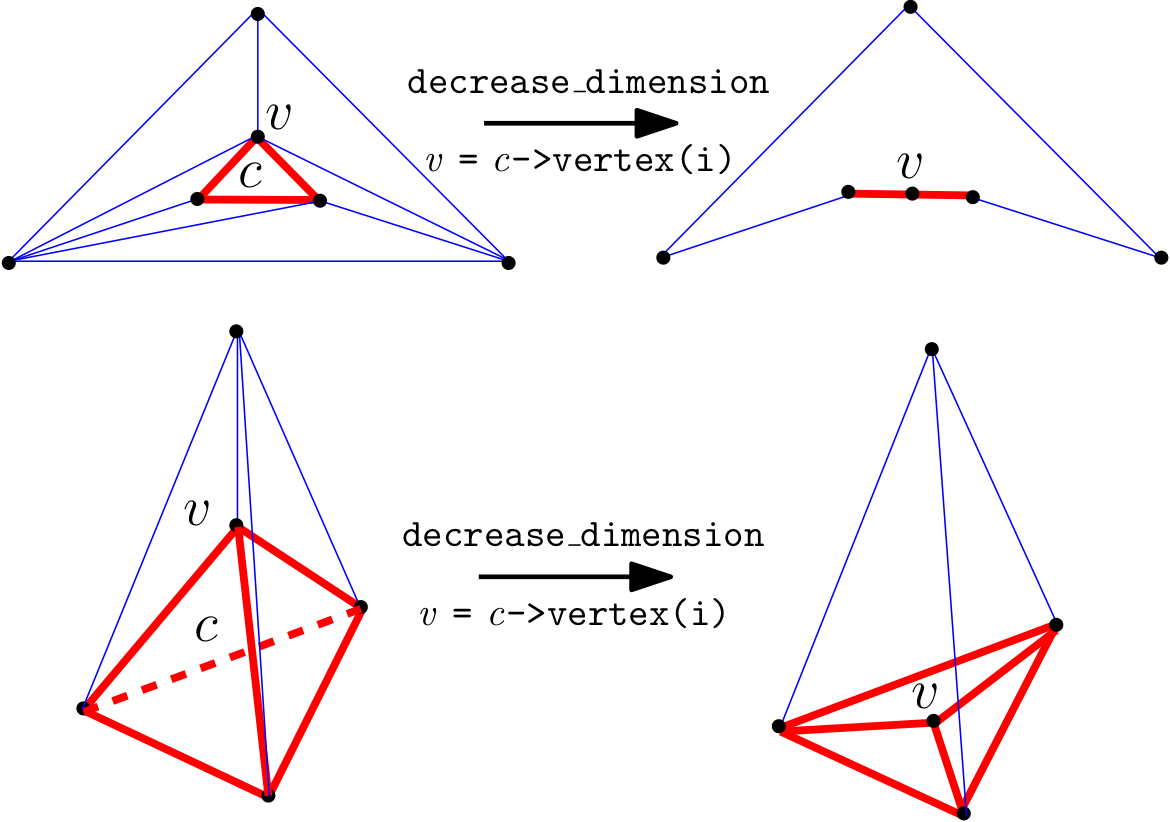
\includegraphics[width=1.0\textwidth]{TDS_2_ref/tds-dim_down}
\end{center}
\end{ccTexOnly} 
\caption{From a two-dimensional data structure to a one-dimensional data structure.}
\label{fig-tds-dim_down_2}
\begin{ccHtmlOnly}
<CENTER>
<img border=0 border=0 height="200" src="./tds-dim_down.png" align=middle alt="From a two-dimensional data structure to a one-dimensional data structure.">
</CENTER>
\end{ccHtmlOnly} 
\end{figure}


\begin{ccAdvanced}
The following modifiers are required for convenience of the advanced
user.
They do not guarantee the combinatorial validity 
of the resulting triangulation.

\ccThree{Vertex_handle}{tds.star_hole( FaceIt face_begin,}{}
\ccMethod{ template< class EdgeIt>
   Vertex_handle  star_hole(EdgeIt edge_begin,EdgeIt edge_end);}
{creates a new vertex \ccc{v} and use it to star the hole 
whose boundary is described  by the sequence of edges \ccc{[edge_begin, 
edge_end[}. Returns a pointer to the  vertex.}
\ccGlue 
\ccMethod{   template< class EdgeIt, class FaceIt>
   Vertex_handle  star_hole(EdgeIt edge_begin, 
                    EdgeIt edge_end,
                    FaceIt face_begin,
                    FaceIt face_end);}
{ same as above, except that, to build the new faces, the  algorithm 
first recycles faces in the sequence \ccc{[face_begin, 
face_end[} and create new ones when the sequence is exhausted.}
\ccGlue
\ccMethod{   template< class EdgeIt>
 void  star_hole(Vertex_handle  v, EdgeIt edge_begin,  EdgeIt edge_end);}
{uses vertex v to  star the hole 
whose boundary is described  by the sequence of edges\ccc{[edge_begin, 
edge_end[}.
}
\ccGlue
\ccMethod{   template< class EdgeIt, class FaceIt>
   void  star_hole(Vertex_handle  v,
                  EdgeIt edge_begin, 
                  EdgeIt edge_end,
                  FaceIt face_begin,
                  FaceIt face_end);}
{same as above, recycling faces in the sequence  \ccc{[face_begin, 
face_end[ . } }

%\ccMethod{Vertex_handle  star_hole(List_edges& hole);}
%{create a new vertex \ccc{v} and use it to star the hole \ccc{hole}.}
%\ccGlue
%\ccMethod{void star_hole(Vertex_handle  v, List_edges& hole);}
%{stars the hole \ccc{hole} using vertex \ccc{v}.}
\ccGlue
\ccMethod{void make_hole(Vertex_handle  v, List_edges& hole);}
{removes the vertex v, and store in \ccc{hole} the list of edges
on the boundary of the hole.}

\ccMethod{Vertex_handle  create_vertex();}{adds a new vertex.}
\ccGlue
\ccMethod{Face_handle create_face(Face_handle f1, int i1, Face_handle f2, int i2, Face_handle
f3, int i3);}{adds a face which is the neighbor \ccc{i1} of \ccc{f1}, 
\ccc{i2} of \ccc{f2} and \ccc{i3} of \ccc{f3}.}
\ccGlue
\ccMethod{Face_handle create_face(Face_handle f1, int i1, Face_handle f2, int i2);}
{adds a face which is the neighbor \ccc{i1} of \ccc{f1}, 
and the neighbor \ccc{i2} of \ccc{f2}.}
\ccGlue
\ccMethod{Face_handle create_face(Face_handle f1, int i1, Vertex_handle  v);}
{adds a face which is the neighbor \ccc{i1} of \ccc{f1},
and has \ccc{v} as vertex.}
\ccGlue
\ccMethod{ Face_handle create_face(Vertex_handle  v1, Vertex_handle  v2, Vertex_handle  v3);}
{adds a face with vertices \ccc{v1}, \ccc{v2} and \ccc{v3}.}
\ccGlue
\ccMethod{Face_handle create_face(Vertex_handle  v1, Vertex_handle  v2, Vertex_handle  v3,
                    Face_handle f1, Face_handle f2, Face_handle f3);}
{adds a face with vertices \ccc{v1}, \ccc{v2} and \ccc{v3},
and neighbors \ccc{f1}, \ccc{f2}, \ccc{f3}.}
\ccGlue
\ccMethod{Face_handle create_face();}
{adds a face whose vertices and neighbors are set to NULL.}
 \ccGlue
\ccMethod{void  delete_face(Face_handle );}{deletes a face.}
\ccGlue
\ccMethod{void  delete_vertex(Vertex_handle );}{deletes a vertex.}
\end{ccAdvanced}



\ccHeading{Miscellaneous}

\ccMethod{int ccw(int i) const;}{returns $i+1$ modulo 3.\ccPrecond $0\leq i \leq 2$.}
\ccGlue
\ccMethod{int cw(int i) const;}
{returns $i+2$ modulo 3.\ccPrecond $0\leq i \leq 2$.}
\ccGlue
\ccMethod{bool is_valid();}{checks the combinatorial validity of the
triangulation: call the \ccc{is_valid()} member function for each vertex and 
each face, checks the number of vertices and the Euler relation
between numbers of vertices, faces and edges.}
\ccGlue
\ccMethod{size_type degree(Vertex_handle v) const;}
{Returns the degree of \ccc{v} in the triangulation.}

\ccHeading{I/O}

The information output  in the \ccc{iostream} is: 
the dimension, the number of (finite) vertices, 
the number of (finite) faces.
Then comes 
for each vertex, the non combinatorial information stored in  that vertex
if any.
Then comes 
for each faces,  the indices of its vertices and 
the non combinatorial information (if any) stored in  this face.
Then comes 
for each face again 
 the indices of the neighboring faces. 
The  index of an item  (vertex of face)
the rank of this item in the output order.
When dimension $<$ 2, the same information is output
for faces of maximal dimension instead of faces.


\ccThree{Vertex_handle}{tds.file_output( ostream& os)}{}
\ccFunction{void tds.file_output( ostream& os,
                   Vertex_handle v = Vertex_handle(),
                   bool skip_first=false);}
{writes \ccVar\ into the stream \ccc{os}. 
If \ccc{v} is not a null handle, vertex \ccc{v}
is output first or skipped if \ccc{skip_first} is true.}

\ccFunction{Vertex_handle tds.file_input( istream& is, 
                           bool skip_first=false);}
{inputs \ccVar\ from file and returns a pointer to the first input vertex.
  If \ccc{skip_first} is true, it is assumed that the first
   vertex has been omitted when output.}

\ccFunction{istream& operator>>
        (istream& is, TriangulationDataStructure_3 & tds);}
{reads a combinatorial triangulation from \ccc{is} and assigns it to \ccc{tds}}

\ccFunction{ostream& operator<<
        (ostream& os, const TriangulationDataStructure_3 & tds);}
{writes \ccc{tds} into the stream \ccc{os}}




\ccHasModels
\ccc{CGAL::Triangulation_data_structure_2<Vb,Fb>} \\

\ccSeeAlso
\ccc{TriangulationDataStructure_2::Face} \\
\ccc{TriangulationDataStructure_2::Vertex} \\
\ccc{CGAL::Triangulation_2<Traits,Tds>}

\end{ccRefConcept}

% +------------------------------------------------------------------------+
%%RefPage: end of main body, begin of footer
% EOF
% +------------------------------------------------------------------------+

